
%(BEGIN_QUESTION)
% Copyright 2011, Tony R. Kuphaldt, released under the Creative Commons Attribution License (v 1.0)
% This means you may do almost anything with this work of mine, so long as you give me proper credit

Read and outline the ``Analog Input References and Connections'' subsection of the ``Analog Signal Conditioning and Referencing'' section of the ``Digital Data Acquisition and Networks'' chapter in your {\it Lessons In Industrial Instrumentation} textbook.  Note the page numbers where important illustrations, photographs, equations, tables, and other relevant details are found.  Prepare to thoughtfully discuss with your instructor and classmates the concepts and examples explored in this reading.

\underbar{file i00884}
%(END_QUESTION)





%(BEGIN_ANSWER)


%(END_ANSWER)





%(BEGIN_NOTES)

{\it Ground-referenced} voltage signals have one pole common with earth or chassis ground.  {\it Floating} voltage signals have neither side connected to ground, but may ``float'' to any potential from ground.  {\it Elevated} voltage signals have a definite common-mode voltage present.  {\it Center-grounded} voltage signals have a common-mode voltage equal to one-half the signal voltage.

Connecting a single-ended DAQ to a ground-referenced voltage signal works over short distances, but over long distances this may cause noise to be picked up through ground path.  Adding a bonding wire just creates a ground loop -- a very bad thing in a signal circuit!  Single-ended DAQs work just fine to measure floating voltage sources, regardless of distance, because the DAQ's ground reference makes the source float no longer.

Differential-input DAQ units are more versatile, able to handle ground-referenced as well as elevated signal sources with ease.  So long as the common-mode limits of the DAQ are not exceeded, it will work even when measuring multiple signal sources.  A limitation of differential-input DAQs is that a ground path must exist somewhere in the input circuit to accommodate the instrumentation amplifier's bias current.









\vskip 20pt \vbox{\hrule \hbox{\strut \vrule{} {\bf Suggestions for Socratic discussion} \vrule} \hrule}

\begin{itemize}
\item{} A problem with resistance-based temperature sensors is a phenomenon known as {\it self-heating}.  Explain how a sensor such as an RTD might heat itself, and how this would affect its ability to precisely and accurately measure temperature.
\item{} Explain why we might wish to build a bridge circuit for measuring temperature with an RTD, rather than the simpler series circuit shown at the beginning of this section.
\item{} Calculate the magnitude of $V_{common}$ when the bridge circuit is balanced with equal-value resistors in all arms of the bridge.  
\item{} What is meant by the expression, ``All grounds are not created equal''?
\item{} Explain how the ground noise voltage problem of the single-ended DAQ application could be overcome if we added an instrumentation amplifier to the circuit.
\item{} Explain how we could tell whether or not we were dealing with significant noise voltage in a single-ended DAQ application, using simple test equipment (e.g. no oscilloscope).
\item{} Explain why the single-ended DAQ has trouble interpreting the signal from an RTD bridge circuit.
\item{} Explain why the two-channel solution would work to measure the signal from an RTD bridge circuit.
\item{} Explain why bias resistors should be very large (and equal!) in value.
\item{} Identify a differential DAQ application where we would only need one bias resistor per channel instead of two.
\item{} Read through the ``essential rules'' listed at the end of this text, explaining the rationale for each one.
\end{itemize}








\vfil \eject

\noindent
{\bf Prep Quiz:}

Explain what a {\it floating} voltage signal is.  Be as specific as you can in your answer, and feel free to cite a realistic application if it helps your explanation.









\vfil \eject

\noindent
{\bf Summary Quiz:}

Identify the problem in the following data acquisition circuit:

$$\includegraphics[width=15.5cm]{i00884x01.eps}$$

%INDEX% Reading assignment: Lessons In Industrial Instrumentation, Digital Data Acquisition and Networks (analog input references and connections)

%(END_NOTES)


